\section{The answer: two channels, measured separately}
\label{sec:channels}

Every two-arm design in this note fails for the same reason --- Direct differs
from Composite in two ways at once, and no choice of $g$ separates them. But
the separation does not have to come from choosing $g$. It can be computed.

\paragraph{Three posteriors, not two.} Alongside the two models we have been
comparing, put a third: the composite prior on $\mathbf h$, conditioned on the
objective values only.

\begin{center}
\begin{tabular}{llll}
\toprule
 & Prior & Conditions on & \\
\midrule
Model 1 & GP on $f$, fitted & $F$ & \emph{Direct} \\
Model 3 & GP on $\mathbf h$, known & $F$ & \\
Model 2 & GP on $\mathbf h$, known & $H$ & \emph{Composite} \\
\bottomrule
\end{tabular}
\end{center}

\noindent Models 1 and 3 see \emph{the same data} and differ only in the
model, so the distance between them is misspecification alone. Models 2 and 3
share \emph{the same model} and differ only in what is observed, so the
distance between them is information alone. The two channels are separated by
construction rather than by hoping two functions are comparable.

For a finite-fiber $g$ all three are computable exactly by enumerating
plausible histories (Section~\ref{sec:exactposteriors}), so this needs no sampler, no
fitting and no replicates.

\paragraph{Result.} Across the root-spread family, at $n=8$ observed points and
12 query points:

\begin{center}
\small
\begin{tabular}{lrrrr}
\toprule
 & & Information & Misspecification & \\
Map & $\bar n$ & $\sup|M_2-M_3|$ & $\sup|M_1-M_3|$ & $I(y;h)$ bits \\
\midrule
\texttt{spr3s000} \ ($=z^3$) & $1.00$ & $\mathbf{0.0000}$ & $0.364$ & $0.000$ \\
\texttt{spr3s025} & $1.88$ & $0.0018$ & $0.380$ & $0.021$ \\
\texttt{spr3s050} & $2.51$ & $0.0670$ & $0.375$ & $0.032$ \\
\texttt{spr3s075} & $2.82$ & $0.1328$ & $0.239$ & $0.027$ \\
\texttt{spr3s100} & $2.96$ & $0.0615$ & $0.261$ & $0.040$ \\
\midrule
\texttt{spr5s000} \ ($=z^5$) & $1.00$ & $\mathbf{0.0000}$ & $0.403$ & $0.000$ \\
\texttt{spr5s025} & $2.33$ & $0.0271$ & $0.428$ & $0.061$ \\
\texttt{spr5s050} & $3.39$ & $0.0192$ & $0.433$ & $0.047$ \\
\texttt{spr5s075} & $4.06$ & $0.1357$ & $0.365$ & $0.055$ \\
\texttt{spr5s100} & $4.50$ & $0.0869$ & $0.267$ & $0.071$ \\
\midrule
\texttt{spr4s000} \ ($=z^4$) & $2.00$ & $0.0979$ & $0.309$ & $0.018$ \\
\texttt{spr4s100} & $3.93$ & $0.0720$ & $0.350$ & $0.031$ \\
\texttt{spr6s000} \ ($=z^6$) & $2.00$ & $0.0911$ & $0.347$ & $0.023$ \\
\bottomrule
\end{tabular}
\end{center}


\begin{figure}[htbp]
\centering
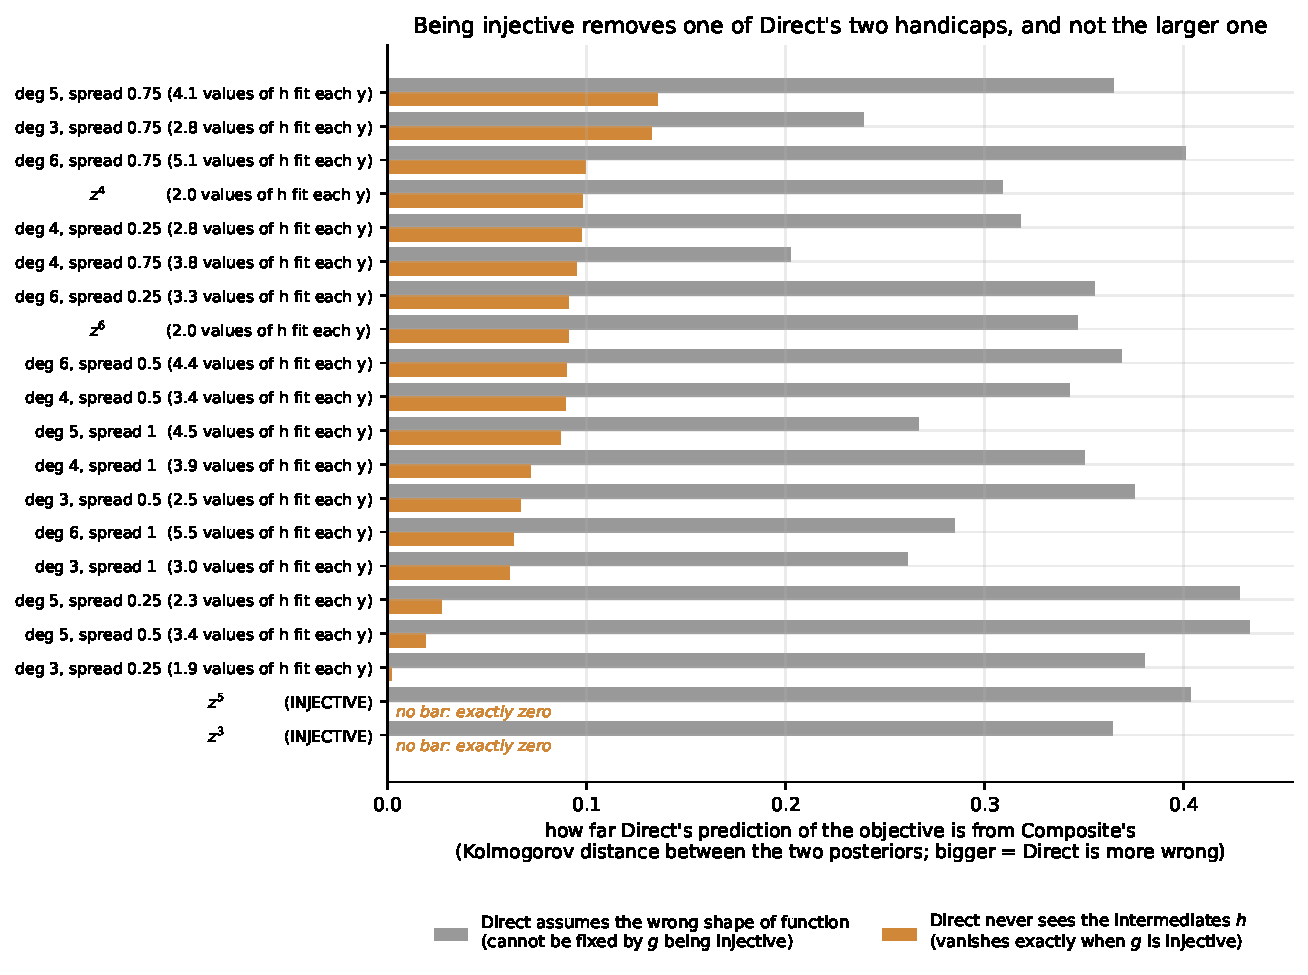
\includegraphics[width=0.86\linewidth]{../figures/channels_simple.pdf}
\caption{The whole result. Grey is how far Direct's prediction sits from
Composite's because it is fitting the wrong shape of model; orange is how far
because it is missing information. The two injective maps have no orange bar
at all --- exactly zero, as the proposition requires --- and their grey bar is
as long as anyone's.}
\label{fig:channels}
\end{figure}

\paragraph{Bijectivity controls the information channel exactly.} It is
$0.0000$ for $z^3$ and $z^5$, the two injective members, and non-zero
everywhere else. The even-degree maps at $s=0$ are $z^4$ and $z^6$, which fold
at the origin and so are \emph{not} injective --- and they duly show
information, $0.098$ and $0.091$. The zeros appear exactly where injectivity
does, independent of degree. This is the proposition, confirmed without a
single fitted model.


\begin{figure}[htbp]
\centering
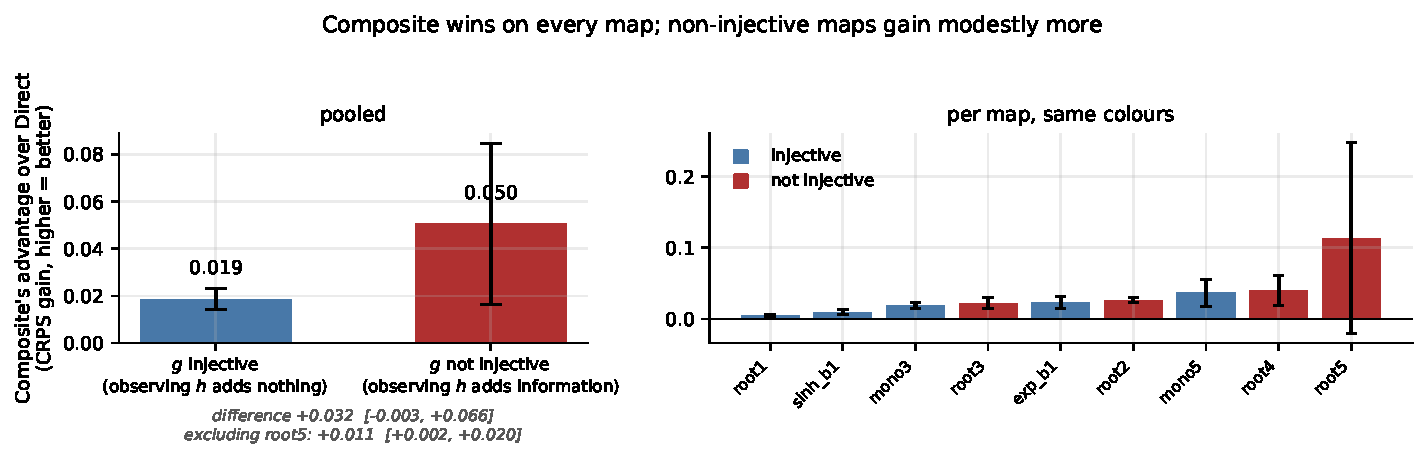
\includegraphics[width=\linewidth]{../figures/gain_grouped.pdf}
\caption{The practical quantity: how much better Composite predicts than
Direct, with the maps pooled by injectivity. Composite wins on every map,
injective or not. The non-injective group does gain more, but modestly, and
the raw gap is inflated by \texttt{root5}, whose own interval spans
zero.}
\end{figure}

\paragraph{But it is the smaller channel.} Misspecification runs $0.24$ to
$0.43$ throughout, including at $s=0$ where there is no information to be had
at all. It is three to seven times the information term and shows no
dependence on injectivity.

That is why the measured Composite-versus-Direct advantage does not track
bijectivity: bijectivity governs the smaller of two terms, and the larger one
is indifferent to it.

\paragraph{The effect looks binary, not graded.} Within the even-degree rows
the information term is nearly flat as $\bar n$ climbs --- degree 4 gives
$0.098, 0.098, 0.090, 0.095, 0.072$ while $\bar n$ goes $2.00$ to $3.93$. What
matters is whether $g$ is injective at all, not how many preimages it has. The
proposition is a binary statement, and the measurement agrees.

\paragraph{What this costs.} The enumeration is exact but noise-free, at
$n=8$ ($n=7$ for \texttt{spr5s100}, to stay tractable). The \emph{zeros} are
exact and hold for any $n$. The magnitudes of the non-zero entries are
specific to this sample size and should not be read as the value of
information in general; what is robust is their ordering against the
misspecification column.
